%%
%% Copyright Guy Taylor 2012
%%
%%

\chapter{Introduction}

\section{Introduction}

The concept of medical equipment that enables unobtrusive wireless monitoring of various human
life-signs has been a recurring theme in science fiction for years\cite{StarTrekStarFleetTechnicalManual1986}, but only recently have
technological advancements been made that might help realize these possibilities and bring them to
market. Realizing the dream of detecting medical conditions early, even before they produce readily-detectable
symptoms, in people fit or ill entails both continuous monitoring of all vital signs (such as
pulse, respiratory rate and temperature) and their analysis in relation to known conditions or
detection trends over the person’s life. This possibility has sparked initiatives such as a 10 million
dollar prize for a "Tricorder"\cite{XprizeHealth2012} and new research into ways of measuring and analysing vital
signs.


In order for the researchers and medical staff to fully achieve these aims, hardware designers and
programmers need to produce platforms that are unobtrusive, easy-to-use and of low cost. A new
generation of devices and technologies are being designed and perfected as part of the research
process to system development, incorporating features such as the latest generation of low-power
\ac{MCU} and wireless transceivers suitable both for patient-monitoring devices
and, in a broader context, for small  consumer-electronics fitness aids\cite{Jawbone2012, Fitbit2012}.

\begin{wrapfigure}{r}{0.5\textwidth}
  \vspace{-10pt}
  \begin{center}
    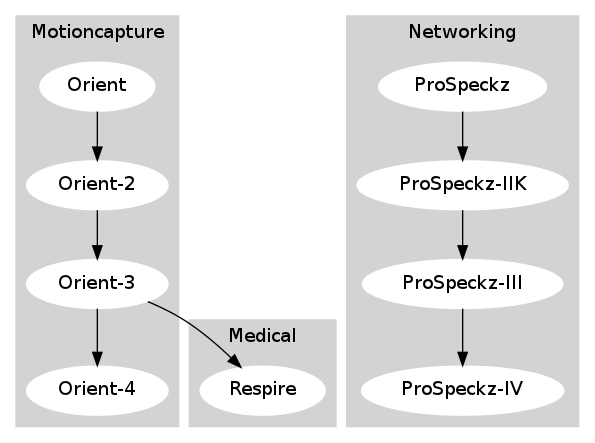
\includegraphics[width=0.4\textwidth, keepaspectratio=true]{images/respire_family_history.png}
  \end{center}
  \caption{Respire family history}
  \vspace{-10pt}
\end{wrapfigure}

The Centre for Speckled Computing within the School of Informatics, University of
Edinburgh, has produced several generations of small low-power sensor platforms for use
in motion capture and general research. These Orient\cite{Orient2012} and ProSpeckz\cite{ProSpeckz2012} devices
have facilitated hardware development and research, embracing the rapid prototype
design methodology. Building on the success of research projects with these devices, it
became apparent that more specific versions were needed both to enable new research and to
reduce the limitations of such a generic platform. This requirement, linked to the rapid development
of suitable microelectronics, has led to the production of two new devices built in tandem. These are
(1)The Respire, a respiratory monitoring device inspired by the Orient-3 motion-capture platform
but built from the ground up for low-power in a smaller, lighter package and (2) the new Orient-5,
upgrading the Orient motion-capture series to the latest generation of technology.

\section{Respiratory Monitoring}

\begin{wrapfigure}{r}{0.3\textwidth}
  \vspace{-10pt}
  \begin{center}
    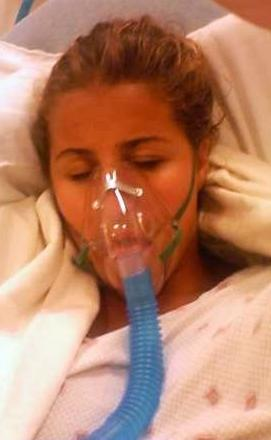
\includegraphics[width=0.2\textwidth, keepaspectratio=true]{images/Plastic_oxygen_mask_on_an_ER_patient.jpg}
  \end{center}
  \caption[Face Mask]{Face mask \cite{FaceMaskImg}}
  \vspace{-10pt}
\end{wrapfigure}

\subsection{Measurement of Respiratory Airflow}
At present the most effective and widely used systems for continuous respiratory monitoring in
people require the patient (or interested subjects) to wear a nasal cannula or face mask and directly
measure respiratory airflow. However, when not necessary for the medical administration of gasses,
these systems are both invasive and uncomfortable for the patient\cite{NasalCannula2011}. Whilst accurate, they
restrict patient movement and are unlikely to be used for long periods of time for monitoring alone.
It has however been demonstrated that an adaptation of the Respire accelerometer-based device
fitted to a nasal cannula could produce a workable wireless monitoring system.

\begin{wrapfigure}{l}{0.3\textwidth}
  \vspace{-10pt}
  \begin{center}
    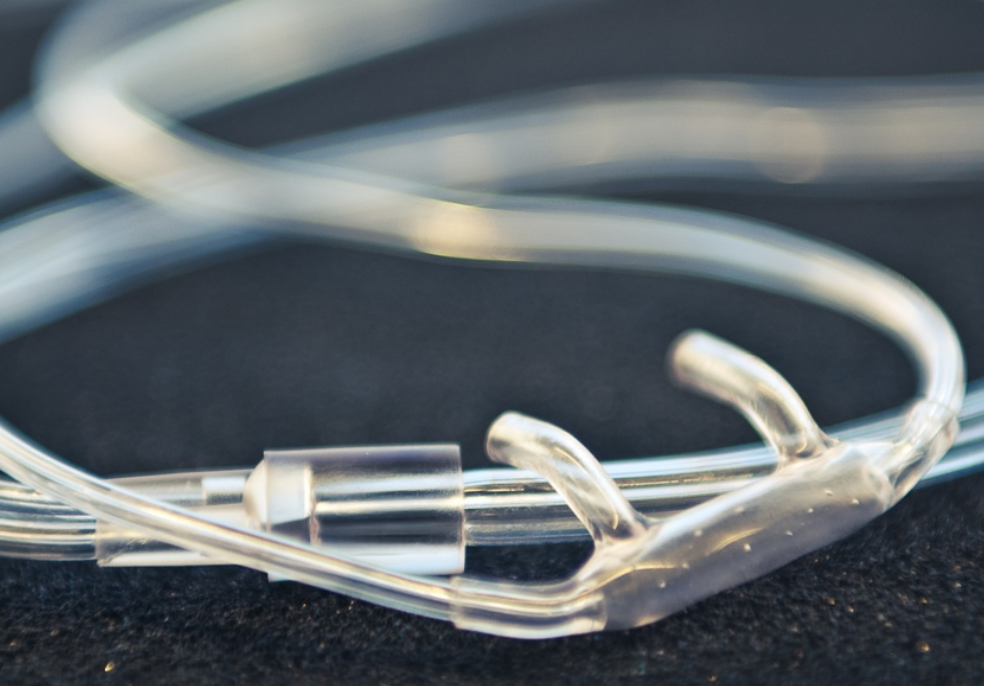
\includegraphics[width=0.2\textwidth, keepaspectratio=true]{images/nasal_canula.png}
  \end{center}
  \caption[Face Mask]{Nasal cannula \cite{SpecknetFlyer}}
  \vspace{-10pt}
\end{wrapfigure}

\subsubsection{Diaphragm Rotation}
The correlation between the rotation of the diaphragm (as measured by acceleration) and the
respiratory rate was recently shown to be accurate enough for medical use by the University of
Edinburgh team who designed the Respire device \cite{BatesLingMannArvind2010}. This non-invasive
means to measure the respiratory rate is achieved by affixing a small accelerometer onto
the patient's lower chest.


\subsubsection{\acf{ECG}}
It is also been shown that single or multiple lead \ac{ECG} can give a reasonable indication of respiratory
frequency ($\pm4$ breaths a minute) and is more independent of the wearer's movements than
accelerometers \cite{ZhaoZhaoQun2008, BoyleBidargaddiSarelaKarunanithi2009}.

\subsection{Usages}
Currently the main use of continuous respiratory monitoring is in intensive
care wards. In respiratory wards there is mainly only the use of non-continuous
60-second breath count measurements with the noting of breathing depth only in vague
terms \cite{Hunter2008}. It however is an increasing field of study, as with the availability of continuous measuring
devices, new diagnostics can be found. This mirrors the previous evolution of other medical
monitoring devices such as heart rate monitors and blood glucose analyzers.
% TODO (COPD ?) %
An example of the potential diagnostic power and applications of continuous respiratory
monitoring is in Sleep Apnoea. With real-time data collection, professionals can quickly diagnose the
condition whilst the patients can be alerted of their onset, thus preventing harm by waking up (ref). % TODO
For this to be successful the system must be unobtrusive enough to
sleep with and be reliable enough to be life-critical.
The overall goal of this project is to support the role of the medical
professionals and research staff in their attempts to find more
effective, comfortable and cheaper ways to diagnose and manage
respiratory conditions. To this end, the devices and designs are there specifically to enable this
purpose and not to break ground in other areas.
To enable collection of continuous respiratory rates, a device that can record and transmit
respiratory data wirelessly whilst still being small and light enough to be carried by the patient is
required. The device should be unobtrusive and simple to use, whilst decreasing the complexity of
the current system. This device should be suitable for use in hospitals at the required technical and
hygiene standards, in an environment that may contain multiple Respire devices and other
electronically controlled systems

\section{Goal}
This project proposes one solution for a new low power radio interface for the Respire device to
facilitate the more general use in a clinical setting.


